% Partie 1.3 - 6LoWPAN %

\subsection{6LoWPAN}

Cette partie à pour but de présenter le protocole 6LoWPAN ainsi que la norme 802.15.4 utilisée dans les couches basses de 6LoWPAN.

\subsubsection{802.15.4}

Ce standard de l'\textbf{IEEE} est définie sur deux couches du \textbf{modèle OSI} : la couche physique et la couche MAC. Il est à la base de différents protocoles IoT (notamment ZigBee) qui implémentent des couches supérieures différentes. 

Le framework de base prévoie un rayon de communication de dix mètres pour un débit allant jusqu'à 250 kbit/s. Il est bien sûr possible de réduire la puissance d'émission (le rayon) et de diminuer le débit pour réduire la consommation électrique. L'idée derrière cette réduction drastique est de quand même de conserver une bonne fiabilité.

Comme Wi-Fi (802.11), 802.15.4 utilise comme méthode d’accès \textbf{CSMA/CA} au niveau 2 pour éviter les collisions et intègre plusieurs mécanisme pour la sécurisation des communications. Certains appareils peuvent aussi intégrer des modules d'optimisation de la consommation, de détection de la qualité de la liaison ainsi que la puissance de réception. 

Les appareils conformes à la norme 802.15.4 peuvent désormais utiliser trois bandes de fréquences : 868, 915 et 2~450 MHz.

Le standard défini deux types de nœud :

\begin{description}
	\item[les \textit{Full-Function Devices} (FFD)] peuvent aussi bien servir de coordinateur dans le PAN que comme nœud simple. Ils sont doté d'un module de communication qui permet de retransmettre des trames (faire du routage) ;
	\item[les \textit{Reduced-Function Devices} (RFD)] sont prévues pour être extrêmement simples et possèdent peu de ressources. À cause de cela, il ne peuvent que communiquer avec les FFD et ne peuvent pas être les coordinateurs.
\end{description}

\subsubsection{6LoWPAN}



\begin{figure}[h]
\centering
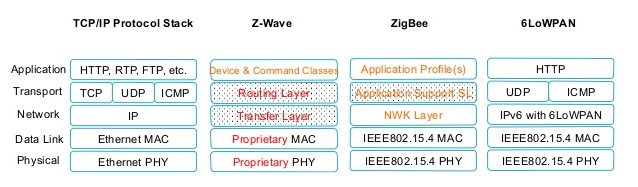
\includegraphics[width=15cm]{\rpDossier/images/comparison.jpg}
\caption{Comparaison de différents protocoles IoT}
\label{comparison}
\end{figure}
